%Balíčky
\documentclass[a4paper,11pt,twoside]{article}
\usepackage[utf8]{inputenc} %kodovani, abychom mohli jednoduse psat diakriticka pismena
\usepackage[czech]{babel}
\usepackage{pifont}
\usepackage{graphicx} %pro vkladani obrazku
\usepackage{color}
\usepackage{fancyhdr} %zahlavi a zapati
\usepackage{ifpdf}
\usepackage{booktabs}
\usepackage{amssymb}
\usepackage{subfigure}
\usepackage{titlesec}
\usepackage[multiple]{footmisc}
\usepackage[final]{pdfpages}    % pro vkládání PDF souborů
\usepackage{pdflscape}   % pro sazbu stránek naležato
\usepackage{color}       % pro zvýraznění textu barvou
\usepackage{multirow} 
\usepackage{amsmath}
\usepackage{sectsty}
\usepackage[justification=centering]{caption}
\usepackage[top=1.5cm, left=3cm, right=3cm, bottom=2cm, headheight=26pt, includeheadfoot]{geometry}
\usepackage[colorlinks=false,urlcolor=black]{hyperref}
\usepackage{xcolor}
\usepackage{listings}
\hypersetup{
    colorlinks=true,
    linkcolor=black,
    filecolor=black,      
    urlcolor=black,
    citecolor=black
}
\allsectionsfont{\rmfamily} 

\sectionfont{\huge}
\subsectionfont{\LARGE}
\subsubsectionfont{\Large}

\def\author{Autoři: Bc. Linda Kladivová, Bc. Jana Špererová}
\def\nazevprace{KONVEXNÍ OBÁLKY}

\begin{document}
\setcounter{page}{1}  % nastaví čítač stránek od stránky Úvod na stránku č. 7
\sloppy
\setlength{\parskip}{1pt}


%%  ÚVODNÍ STRÁNKA %%%%%%%%%%%%%%%%%%%%%%%%%%%%%%%%%%%%%%%%%%%%%%

\pagestyle{empty} % vypne číslování stránek na úvodní straně

\begin{center}
\renewcommand{\baselinestretch}{1.35} %zvetseni mezery mezi radky

\LARGE
\textsc{České vysoké učení technické v~Praze} \\
\textsc{Fakulta stavební} \\

\bigskip

\large
\textsc{PROGRAM GEODÉZIE A KARTOGRAFIE} \\
\textsc{OBOR GEOMATIKA} \\

\vspace{10ex}

\begin{figure}[hbt!] %vlozeni loga
\begin{center}

\includegraphics[width=7cm]{pictures/symbol_cvut_konturova_verze_cb.pdf} 
\end{center}
\end{figure}

\vspace{20ex}

\large
\textsc{\nazevprace} \\
\smallskip


\vspace{6ex}

\normalsize
\textsc{\author} \\
\bigskip
\normalsize
\textsc{Předmět: Algoritmy digitální kartografie a GIS} \\

\end{center}


%% 2. STRÁNKA OBSAHUJE ZADÁNÍ
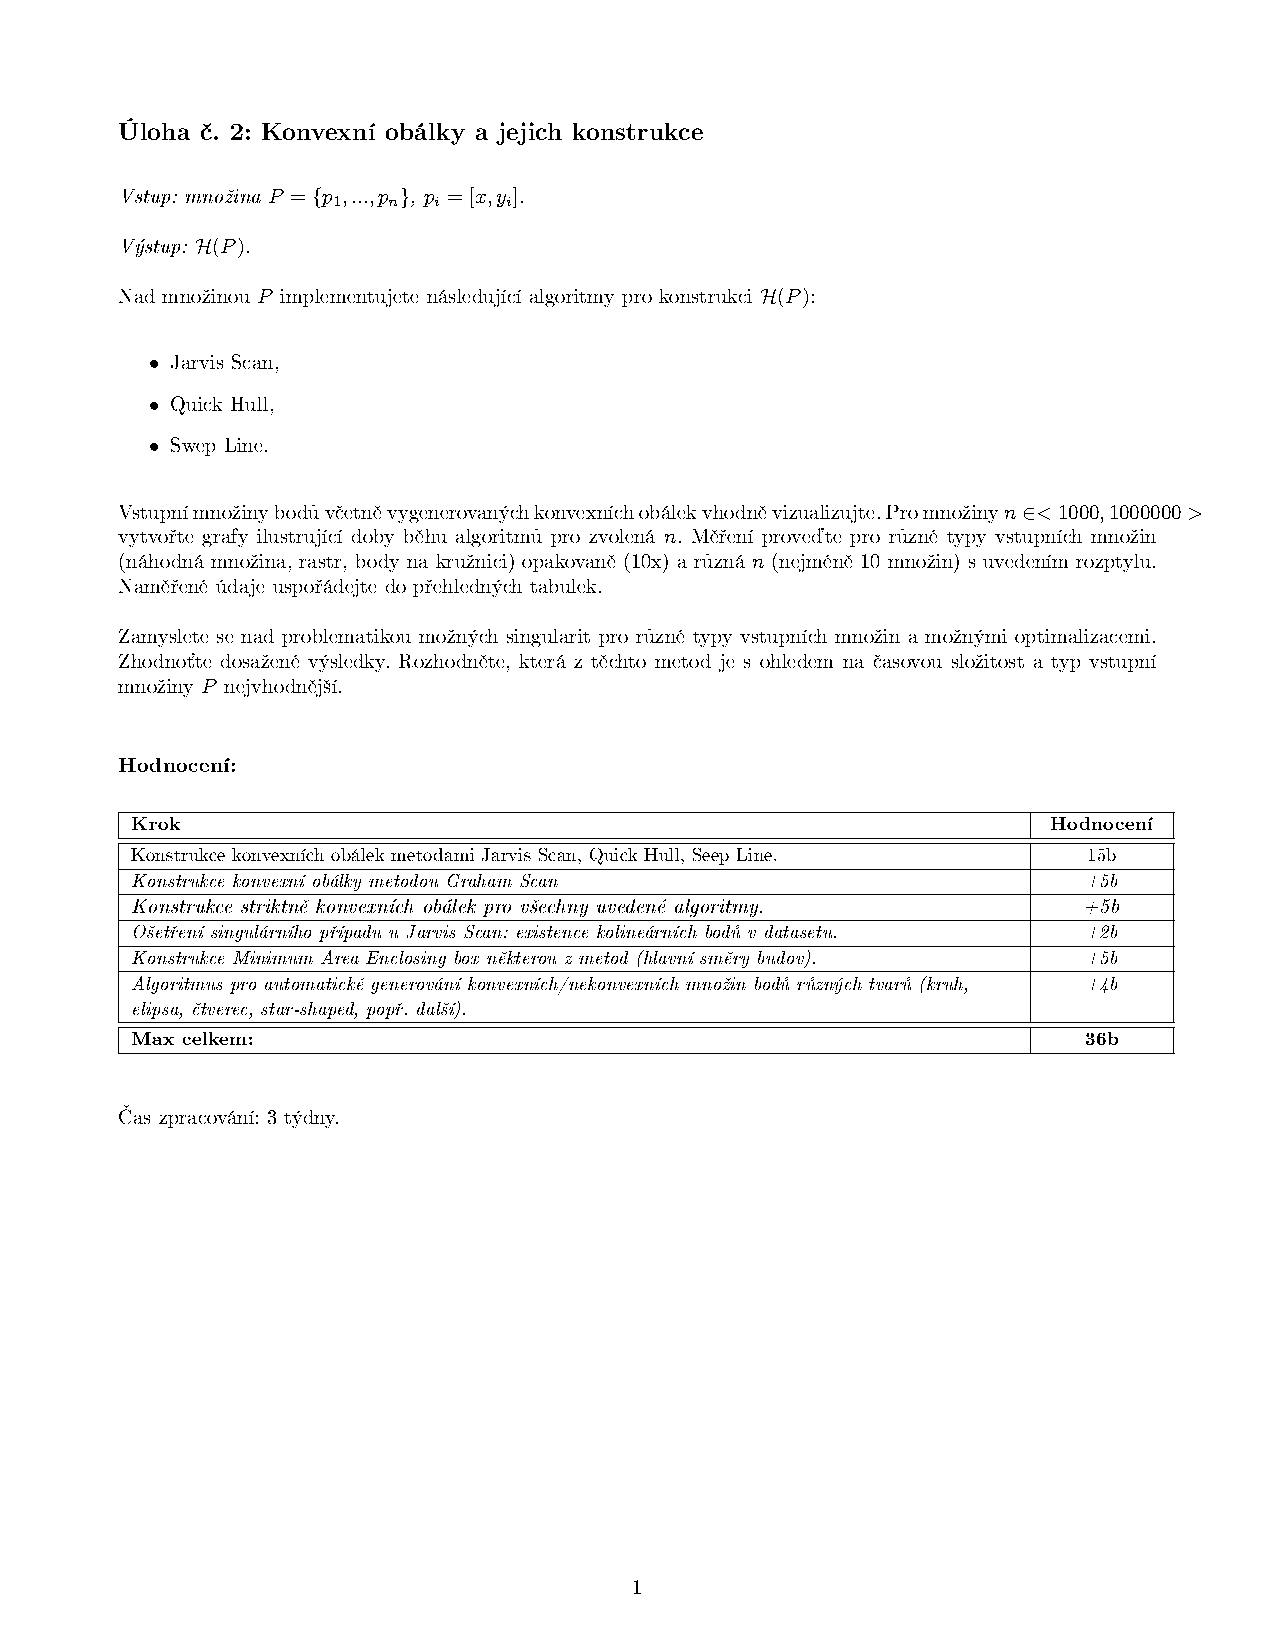
\includepdf{pictures/adkcv2}


%% 3. a 4. STRÁNKA = OBSAH A SEZNAM OBRAZKU %%%%%%%%%%%%%%%%%%%%%%%%%%%%%%%%%%
\renewcommand{\baselinestretch}{1.4} %zvetseni mezery mezi radky
\newpage
\tableofcontents %obsah

\newpage
\listoffigures %seznam obrázků
%\listoftables %seznam tabulek

\thispagestyle{empty}
\newcommand{\obrazek}[1]{(viz obr. \ref{#1})} %specialni reference na obrazek

\newpage
\pagestyle{fancy}

%% NASTAVENI VZHLEDU STRANEK (ZAHLAVI A ZAPATI)

\renewcommand{\baselinestretch}{1.4} %zvetseni mezery mezi radky

% zajistí, že se názvy kapitol a sekcí nebudou sázet velkými písmeny
\renewcommand{\sectionmark}[1]{\markright{\ #1}}

\fancyhf{} % smaže aktuální nastavení záhlaví a zápatí
\renewcommand{\headrulewidth}{0.4pt} % vrchní linka
\renewcommand{\footrulewidth}{0.4pt}  %  spodní linka
\addtolength{\voffset}{-0.4cm}

 %záhlaví
\fancyhead[LE, LO]{{
\includegraphics[width=1cm]{pictures/symbol_cvut_konturova_verze_cb.pdf} }
   {\textsc{\small {ČVUT v Praze}} }} %logo skoly
\fancyhead[RE, RO]{\nouppercase{\rightmark}}
   
 %zápatí
\fancyfoot[RO, LE]{{\textsc{\small \thepage}}}

\fancypagestyle{plain}{
  \fancyhead{} % na prázdných stránkách nechci záhlaví
  \renewcommand{\headrulewidth}{0pt} % ani linku
}


%% -------<<< 1. KAPITOLKA = Popis a rozbor problému >>>-------\\%%

\newpage
\pagestyle{fancy}
\fancyhead[RE, RO]{\fancyplain{}{\small \sl{POPIS A ROZBOR PROBLÉMU}}}

\vspace*{-1cm}
\section{Popis a rozbor problému}
\noindent
\large
Záměrem této úlohy je vytváření konvexních obálek pro libovolné množství vygenerovaných bodů. Konvexní obálka je uzavřená hranice spojující konkrétní body množiny tak, že každý bod množiny se nachází uvnitř nebo na hranici obálky (bod obálky). A také pokud spojíme dva libovolné body množiny úsečkou, tak daná úsečka leží v konvexní obálce nebo je s ní totožná. \\
\indent Konvexní obálky se využívají například v kartografii (natočení budov), v geodézii (3D modelování), u počítačových her (prostředí), v designu či grafice a ve spoustě dalších oborů.

\vspace{0.2cm}
\begin{figure}[hbt!] 
\begin{center}
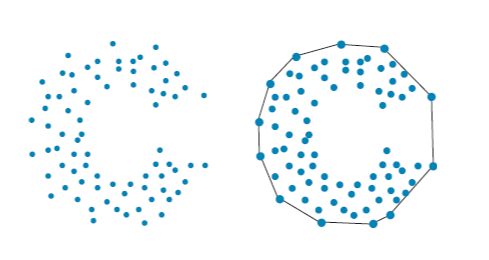
\includegraphics[width=15cm]{pictures/convex.png} 
\caption[Ukázka konvexní obálky nad vstupní množinou bodů]{Ukázka konvexní obálky nad vstupní množinou bodů \cite{convex}}
\label{fig:convex}
\end{center}
\end{figure}
\vspace{-0.4cm}

\subsection{Údaje o bonusových úlohách}
\large
\noindent Byla snaha o to splnit všechny bonusové úlohy. Kromě konstrukce konvexních obálek metodami Jarvis Scan, Quick Hull a Sweep Line, byla naprogramována i konstrukce metodou Graham Scan. Vzhledem k tomu, že bylo zadáním změřit doby trvání algoritmů pro různé typy vstupních množin, byl vytvořen Combo Box s výběrem různých typů množin (kruh, elipsa, grid, čtverec, náhodná množina, star-shaped polygon), jejichž konstrukce byla zvlášť definována v samostatné třídě Generator, která združuje několik funkcí vytvářejících výsledný obrazec na základě předem vybraného počtu bodů a typu množiny. \\
\indent Kromě konstrukce konvexní obálky byl napsán algoritmus pro konstrukci Minimum Area Enclosing Box, který nezobrazuje pouze výsledný box, ale také hlavní směr budovy. \\
\indent V rámci algoritmu Jarvis Scan byla ošetřena existence kolineárních bodů v datasetu. Aby byla výsledná obálka opravdu správně zkonstruovaná, bylo nutné vynechat body, které leží na přímce mezi 2 body konvexní obálky a dále smazat body, které jsou identické s body obálky. K tomuto účelu byla napsána funkce CorrectCH, která je implementována na závěr každého ze zmíněných algoritmů na generování konvexních obálek.

\vspace{0.2cm}
\begin{figure}[hbt!] 
\begin{center}
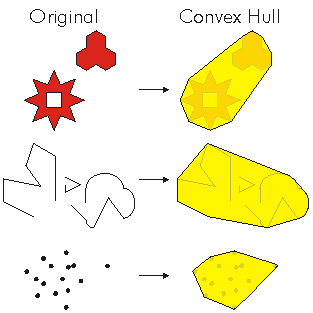
\includegraphics[width=10cm]{pictures/convex2.png} 
\caption[Ukázka konvexní obálky nad různými vstupními množinami]{Ukázka konvexní obálky nad různými vstupními množinam \cite{convex2}}
\label{fig:convex2}
\end{center}
\end{figure}
\vspace{-0.4cm}

%% -------<<< 2. KAPITOLA = Popis použitých algoritmů >>>-------\\%%

\fancyhead[RE, RO]{\fancyplain{}{\small \sl{POPIS POUŽITÝCH ALGORITMŮ}}}
\newpage
\vspace*{-1cm}
\section{Popis použitých algoritmů}
\noindent
\large
Cílem této úlohy je vytvořit aplikaci, která po výběru různého typu vstupní množiny (náhodná množina, rastr, kružnice, star-shaped polygon, elipsa)  vygeneruje automaticky daný obrazec s předem definovaným počtem bodů. Nad tímto obrazcem poté pomocí různých metod zkontruuje konvexní obálku nebo Minimum Area Enclosing Box. V praxi se ke konstrukci konvexních obálek využívá několik různých metod. V této práci byly naprogramovány metody Jarvis Scan, Quick Hull, Sweep Line (zametací přímka) a metoda Graham Scan. Dalšími používanými metodami jsou Divide and Conquer či inkrementální kontrukce. Na dalších řádcích jsou podrobně popsány využité algoritmy pro generování konvexních obálek a také algoritmus hlavních směrů budov, který je využíván při konstrukci Minimum Area Enclosing Box.

\subsection{Jarvis Scan}
\large
Jarvis Scan je metoda, která vyhledává body konvexní obálky na základě hledání maximálního úhlu, tedy předpokládá, že tři body neleží na jedné přímce. Tento algoritmus lze snadno i využít pro prostorové body. Algoritmus pro sestavení metody Jarvis Scan je snadný, avšak časová náročnost tohoto algoritmu je jeho nevýhodou. Jeho rychlost je O(n2) pro body ležící na kružnici, nejběžněji pak O(n*h), kde n je počet bodů vstupní množiny a h je počet bodů konvexní obálky. \\
\indent První bod, ze kterého celý algoritmus vychází, je bod s nejmenší y souřadnicí, někdy také označován jako pivot. Víme, že tento bod bude ležet na konvexní obálce. Tímto bodem povedeme rovnoběžku s osou x a následně projdeme všechny body množiny [i] a změříme úhel mezi rovnoběžkou s osou x a přímkou určenou bodem p (pivot) a i. Tyto úhly mezi sebou porovnáváme a největší z těchto úhlů nám označí následující bod konvexní obálky. V dalším kroku je ošetřena singulární situace, kdy bod s dosavadním maximálním úhlem a současný bod i, leží na jedné přímce, tedy úhly jsou téměř totožné. Pokud se tak stane, je jako dosavadní bod s největším úhlem přídán ten bod, který je vzdálenější od bodu $p_j$. \\
\indent Nyní se nám bod i stává novým pivotem a bod p se stává bodem určující přímku, od které se měří úhly. Takto pokračujeme stále znovu, dokud se bodem i nestane opět bod p.

\newpage
\vspace*{-1cm}
\subsubsection{Slovní zápis algoritmu s ošetřením kolineárních bodů}
\begin{enumerate}
\item Setřídění vstupní množiny bodů podle souřadnice y.
\item Nalezení pivota q:  $ q = min(y_i) $. Pokud nalezeny dva body, vezmi ten s maximální souřadnicí x.
\item Přidej bod q do konvexní obálky:  $ q \rightarrow CH  $ 
\item Nalezení bodu r ve směru osy x (levé rameno úhlu): $ r = (q.x()-1, q.y()) $.
\item Inicializuj: $p_j = q; p_{j-1} = r$
\item Opakuj, dokud: $ p_j \ne q $
\subitem Opakuj pro všechny body vstupní množiny:
\subsubitem Nalezni $p_i$: $ p_i= arg  max_{\forall p_i \in P}  \angle (p_{j-1}, p_j, p_i)$ 
\subsubitem Vypočti  $ dist_i, dist_{imax}$ pokud $ |angle_{max} - angle_{current}| < eps $ 
\subsubitem Pokud je $ dist_i > dist_{imax}$, prohlaš bod $i$, že má maximální úhel
\subitem Přidej vybraný bod $p_i$: $ p_i \rightarrow CH  $
\subitem Přeindexuj body: $ p_{j-1} = p_j; p_j = p_i  $
\end{enumerate}

\vspace{0.2cm}
\begin{figure}[hbt!] 
\begin{center}
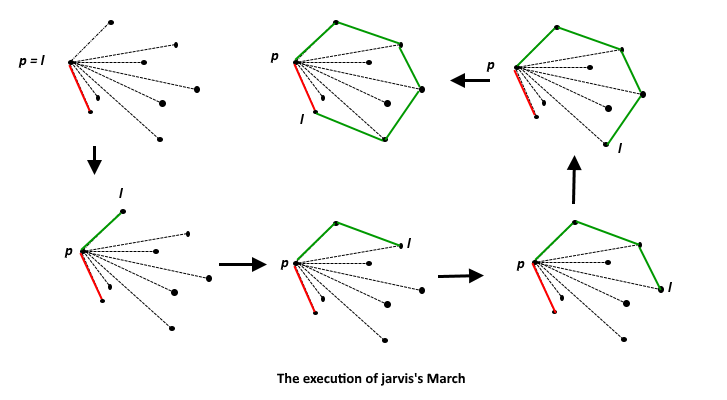
\includegraphics[width=13cm]{pictures/jarvis.png} 
\caption[Princip Jarvis Scan algoritmu]{Princip Jarvis Scan algoritmu \cite{graham}}
\label{fig:graham}
\end{center}
\end{figure}
\vspace{-0.4cm}

\newpage
\vspace*{-1cm}
\subsection{Graham Scan}
Algorithmus Graham Scan funguje na principu zjišťování CCW (levotočivé) orientace trojúhelníku. Algoritmus Graham Scan je velmi rychlý, podobně, jak algoritmus metody Sweep Line, či Quick Hull metody.  Jeho rychlost je O(n*log(n)), kde n je počet bodů vstupní množiny. \\
\indent Na počátku algoritmu setřídíme body podle Y souřadnice a bod s nejmenší Y souřadnicí označíme jako pivot (p). Poté se vypočítá směrnice vzhledem k ose x ke všem bodům množiny. Tyto body pak následně seřadíme podle velikosti směrnice. Následně vždy testujeme CCW orientaci na posledních 2 bodech přidaných do množiny konvexní obálky a poslední bod s největší směrnicí. Takto pak postupujeme analogicky, dokud nenalezneme konvexní obálku. \\
\indent Tato metoda je pojmenována nikoli po tom, jak funguje, ale po Ronaldu Grahamovi, který tuto metodu publikoval roku 1972.


\vspace{0.2cm}
\begin{figure}[hbt!] 
\begin{center}
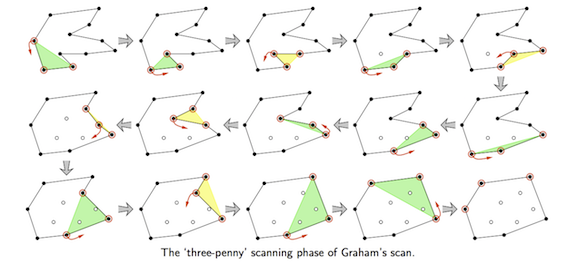
\includegraphics[width=15cm]{pictures/GrahamScan.png} 
\caption[Princip Graham Scan algoritmu]{Princip Graham Scan algoritmu \cite{graham}}
\label{fig:graham}
\end{center}
\end{figure}
\vspace{-0.4cm}

\subsubsection{Slovní zápis algoritmu}
\begin{enumerate}
\item Setřídění vstupní množiny bodů podle souřadnice y.
\item Nalezení pivota q:  $ q = min_{\forall p_i \in S} (y_i), q \in CH $ (pokud jsou souřadnice y u bodů stejné, vybere toho s nejvyšším indexem).
\item Nalezení bodu s ve směru osy x (levé rameno úhlu): $ s = (q.x()-1, q.y()) $.
\item Opakuj pro všechny body vstupní množiny:
\subitem Spočti $omega_i$: $ omega_i= \angle (s, q, p_i)$ 
\subitem Spočti $dist_i$: $ dist_i= |q p_i| $
\item Setřídění bodů dle úhlu s osou x: $ {\forall p_i \in S}$ sort by $ \omega_i = \angle (s, q, p_i)$ 
\item Při nalezení stejného úhlu: $ \omega_k = \omega_l \rightarrow $ neuvažovat bližší bod
\item Vložení prvního bodu s nejmenším úhlem do množiny: $ CH \leftarrow p_1$
\item Opakuj pro všechny setříděné body: $j < n $
\subitem If $ p_j $ vpravo od předešlých bodů $ \rightarrow$ odeber poslední prvek CH
\subitem V opačném případě přidej bod do CH: $ p_{j}  \rightarrow H $
\end{enumerate}

\subsection{Quick Hull}
Quick Hull je metoda, která vyhledává body konvexní obálky, na základě vyhledávání nejvzdálenějšího bodu od přímky, která je určena 2 body množiny bodů. Rychlost algoritmu při použití metody Quick Hull je rychlá O(n*log(n)), ale někdy může dosáhnout i stejné rychlosti, jako při použití algoritmu Jarvis Scan, avšak to nastává jen v nejhorším případě a to O(n2), kde n je počet bodů vstupní množiny. \\
\indent Algoritmus vychází z přímky, která je určena dvěma body množiny bodů. Tyto body, jsou body s nejmenší a největší x souřadnicí. Tato přímka nám množinu bodů rozdělí na 2 poloviny a my v každé polovině procházíme všechny body a zjišťujeme jejich vzdálenost od přímky Xmin Xmax. Když najdeme nejvzdálenější bod od přímky, přidáme ho do konvexní obálky a spojíme s ho s body Xmin Xmax. Tím nám vzniknou další dvě přímky a od nich pokračujeme stále analogicky stejně. Tento postup děláme pro horní množinu bodů i dolní množinu bodů, dokud nevytvoříme konvexní obálku. \\
\indent Tato metoda je také jinak známá jako metoda Divide and Conquer, což v překladu znamená, rozděl a panuj. Naše přímka rozdělí množinu bodů na dvě části a v nich pak hledáme „panující“ bod, ten nejvíce vzdálený.

\vspace{0.2cm}
\begin{figure}[hbt!] 
\begin{center}
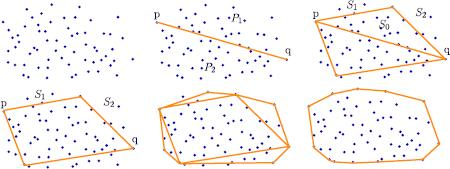
\includegraphics[width=15cm]{pictures/hull2.jpg} 
\caption[Princip dělení  u Quick Hull algoritmu]{Princip dělení  u Quick Hull algoritmu \cite{quick}}
\label{fig:quick}
\end{center}
\end{figure}
\vspace{-0.4cm}

\newpage
\vspace*{-1cm}
\subsubsection{Slovní zápis algoritmu}
\begin{enumerate}
\item Vytvoření horní a dolní množiny:  $upoints = 0; lpoints = 0 $ 
\item Nalezení extrémních hodnot:  $ q_1 =  min_{\forall p_i \in S}(x_i); q_3 =  max_{\forall p_i \in S}(x_i) $ 
\item Přidání extrémních bodů do horní a dolní množiny: $upoints \leftarrow q_1; upoints \leftarrow q_3; lpoints \leftarrow q_1; lpoints \leftarrow q_3 $
\item Pro všechny body množiny: $\forall p_i \in S  $:
\subitem Patří bod do horní množiny? $ if(p_i \in \sigma_l(q_1, q_3)) upoints \leftarrow p_i  $
\subitem V opačném případě: $ lpoints \leftarrow p_i  $
\item Přidání krajního bodu do konvexní obálky: $CH \leftarrow q_3$
\item Nalezení nejvzdálenějšího bodu $c$ v horní části od přímky, přidání do množiny konvexní obálky a opakování vůči nově vzniklé přímce (rekurze)
\item Přidání krajního bodu do konvexní obálky: $CH \leftarrow q_1$
\item Opakování hledání nejvzdálenějšího bodu v dolní části (rekurze)
\end{enumerate}


\newpage
\vspace*{-1cm}
\subsection{Metoda zametací přímky (Sweep Line)}
Sweep Line je metoda, která funguje na principu inkrementální konstrukce, tedy přírůstkové, jelikož mám množinu rozdělenou na část již zpracovanou a tu doplňuji o nové body z nezpracované části, dokud nezpracuji celou množinu bodů. Algoritmus Sweep Line je velmi rychlý, podobně, jak algoritmus metody Quick Hull. Jeho rychlost je O(n*log(n)), kde n je počet bodů vstupní množiny. \\
\indent Algoritmus pracuje s množinami předchůdců a následníků. Na počátku máme seřazené body podle X souřadnic a první dva mezi sebou propojíme, pak se přesuneme na další bod a ten propojujeme s naší úsečkou a určíme jeho předchůdce a jeho následníky. Takto pokračujeme stále dál, dokud nevytvoříme kompletní konvexní obálku.Tato metoda je také známá pod názvem zametací přímka.

\vspace{0.2cm}
\begin{figure}[hbt!] 
\begin{center}
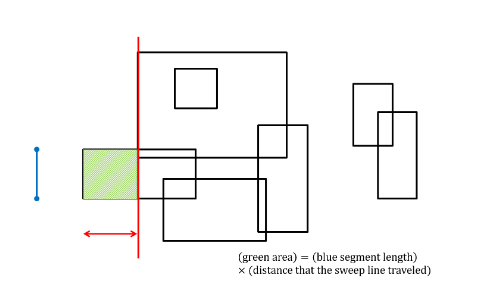
\includegraphics[width=15cm]{pictures/sweep.png} 
\caption[Princip zametací přímky]{Princip zametací přímky \cite{sweep}}
\label{fig:quick}
\end{center}
\end{figure}
\vspace{-0.4cm}

\subsubsection{Slovní zápis algoritmu}
\begin{enumerate}
\item Setřídění bodů množiny podle osy x 
\item Odstranění dupliciticních vstupních bodů
\item Vytvoření vektoru předchůdců a vektoru následovníků
\item Vytvoření počáteční aproximace pomocí dvojúhelníku:  $ n[0] = 1; n[1] = 0; p[1] = 0;  p[0] = 1$
\item Vyhodnocování následujících bodů: $ for~ p_i \in P_S, i \textgreater 3$
\subitem Porovnání hodnoty souřadnice y: $ if (y_i \textgreater y_{i-1})  $
\subsubitem Změna indexů při splnění podmínky: $ p[i] = i-1; n[i] = n[i-1]$
\subsubitem V opačném případě: $ p[i] = p[i-1]; n[i] = i-1$
\subitem Přeindexování $ n[p[i]] = i; p[n[i]] = i  $
\subitem Opravení horní tečny $ while (n[n[i]]) \in \sigma_R (i, n[i]) $:
\subsubitem Změna indexů: $ p[n[n[i]]] = i; n[i] = n[n[i]]$
\subitem  Opravení dolníí tečny $ while (p[p[i]]) \in \sigma_L (i, p[i]) $:
\subsubitem Změna indexů: $ n[p[p[i]]] = i; p[i] = p[p[i]]$
\item Podle vektoru následníků sestav polygon CH
\end{enumerate}

\subsection{Metoda hlavních směrů budov}
Tato metoda vytváří obdélník okolo množiny bodů, který má nejmenší obsah. Princip této metody spočívá v tom, že porovnáváme obdélníky takové, které byly vytvořeny tak, aby minimálně jedna strana konvexní obálky byla totožná se stranou obdélníku.
Časová náročnost této metody je stejná, jako u vytváření konvexní obálky metodou Jarvis Scan. Její rychlost je O(n), kde n je počet bodů vstupní množiny. \\
\indent Na počátku máme konvexní obálku okolo množiny bodů. My nyní vybereme jednu stranu konvexní obálky a tou proložíme první stranu obdélníka. Následně najdeme levé maximum, pravé maximum a horní maximum a vytvoříme obdélník, kde jedna strana je totožná s hranou konvexní obálky a zbylé hrany jsou totožné s minimálně 1 bodem konvexní obálky. Vypočítáme obsah tohoto obdélníka. Takto pokračujeme analogicky, dokud nebudeme mít vypočítané obsahy všech obdélníků nad všemy hranami konvexní obálky. Obsahy pak porovnáme a obdélník o nejmenším obsahu je náš hledaný minimální obdélník.


\vspace{0.2cm}
\begin{figure}[hbt!] 
\begin{center}
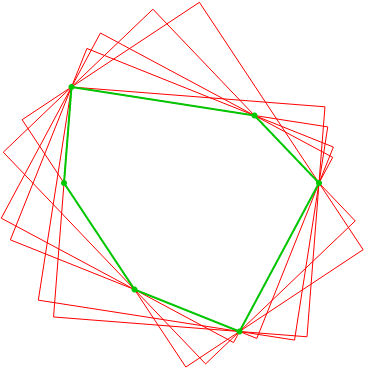
\includegraphics[width=10cm]{pictures/obdelniky.png} 
\caption[Obdélníky při konstrukci Minimum Area Enclosing Box]{Obdélníky při konstrukci Minimum Area Enclosing Box \cite{box}}
\label{fig:box}
\end{center}
\end{figure}
\vspace{-0.4cm}

\subsubsection{Slovní zápis algoritmu}
\begin{enumerate}
\item Inicializuj minimální plochu na velkou hodnotu: $ A_{min} = limit_{double} $
\item Inicializace místního souřadnicového systému a inicializace min a max souřadnic pootočené CH a min max souřadnic Enclosing Boxu 
\item Pro všechny vstupní body CH:
\subitem Převeď do místního systému: $points_i = p; points_{i+1} = k$
\subitem Určií minimální a maximální souřadnice otočené konvexní obálky 
\subitem Nalezni obdélník, který se dotýká konvexní obálky v extrémních bodech
\subitem Porovnej s minimální plochou If $A < A_{min}$: 
\subsubitem $ A_{min} = A; Save (min X, max X, min Y, max Y); Save Angle $
\item Vytvoř obdélník z (min X, max X, min Y, max Y).
\item Nalezni hlavního směru obdélníku v místní soustavě.
\item Transformuj obdélník i hlavní směr budovy do globálního systému o úhel Angle.
\end{enumerate}

\newpage
\vspace*{-1cm}
\subsection{Generátor konvexních/nekonvexních množin bodů různých tvarů}
Generátory jsou naimpementovány jako jednotlivé metody ve třídě Generator. Smyslem aplikace je, aby si mohl uživatel vybrat příslušný tvar - kruh, čtverec, elipsu, grid, náhodné rozmístění či star shaped obrazec, a teprve nad tímto obrazcem mohl konstruovat konvexní obálky, případně Minimum Area Enclosing Box. Náhodné generování bylo implementováno skrze funkce \textit{rand} a \textit{modulo}, aby bylo dosaženo správné zobrazení vygenerovaných bodů uvnitř zobrazovacího okna. \\
\indent Pro tvorbu kruhu byl nejprve náhodně vygenerován střed kružnice a její poloměr. V závislosti na počtu zadaných bodů byl určen středový úhel dvou po sobě jdoucích bodů. Pokud je vstupní počet bodů menší než tři, je zobrazena chybová hláška (ze dvou dobů kružnici nevytvořím). Body na kružnici byly poté vygenerovány ze známých vzorců:
$$ X = X_0 + r.cos(\phi)$$
$$ Y = Y_0 + r.sin(\phi) $$
\noindent Elipsa byla generována obdobně jako kruh s tím rozdílem, že nebyl náhodně generován poloměr, ale hodnoty hlavní poloosy (a) a vedlejší poloosy (b).  Body na elipse byly poté vygenerovány ze známých vzorců:
$$ X = X_0 + a.cos(\phi)$$
$$ Y = Y_0 + b.sin(\phi) $$
\noindent Při tvorbě čtverce je nejprve kontrolováno, zda je počet zadaných bodů opravdu dělitelný čtyřmi. Pokud je menší než čtyři, je zobrazena chybová hláška. Pokud není zadaný počet dělitelný čtyřmi je zobrazena upozorňující hláška a počet generovaných bodů mezi vrcholy čtverce je upraven tak, aby v rámci každé strany čtverce byl generován stejný počet bodů. Prvním vygenerováným náhodně umístěným bodem je levý horní roh. Poté je náhodně určena délka hrany, díky které může jsou dopočteny souřadnice zbývajících vrcholů a také délka krátké úsečky mezi body na hraně. \\
\indent Při tvorbě Star Shaped množiny je automaticky vygenerován střed obou kružnic a poloosy a, b.  Pro polygony typu star shaped je typické, že z jeho středu lze vidět do všech vrcholů. Polovina bodů je tedy vygenerována na kružnici s poloměrem a, druhá polovina na kružnici s poloměrem b, tak aby dva po sobě jdoucí body byly vytvořeny s různou vzdáleností od středu. Pokud je vstupní počet bodů menší než šest, je zobrazena chybová hláška. (Pro tvorbu dvou kružnic se stejným středem a různým poloměrem potřebuji nejméně šest bodů). Body byly vygenerovány ze vzorců:
$$ X_i = X_0 + a * cos(\phi)$$
$$ Y_i = Y_0 + a * sin(\phi) $$
$$ X_{i+1} = X_0 + b * cos(\phi)$$
$$ Y_{i+1} = Y_0 + b * sin(\phi) $$
\noindent Nejjednodušší implementací bylo vytvoření náhodně rozmístěných bodů v rámci okna. Body byly náhodně vygenerovány pomocí funkcí \textit{rand} a \textit{modulo} .
\indent Algoritmus pro tvorbu pravidelné mřížky je v mnoha ohledech podobný algoritmu pro generování množiny čtvercového tvaru. Vzhledem k tomu, že generujeme pravidelnou mřížku, je zapotřebí, aby vstupní počet bodů byl roven nejméně čtyřem a také aby byl druhou mocninou nějakého přirozeného čísla. Pokud druhá podmínka není splněna, je počet bodů redukován pomocí přetypování na integer a uživatel je na změnu upozorněn. Takovýto případ může nastat například při zadání 17 bodů. Odmocnina (v tomto případě rovna $4.12$) je přetypována na integer, tedy na číslo 4. Vytvořený grid má tedy velikost 4 x 4. Levý horní roh mřížky je nastaven napevno na souřadnice (10,10), ostatní body jsou dopočteny podle předem náhodně vygenerovaných délek mezer mezi body v ose x i v ose y.

\begin{figure}[hbt!] 
\begin{center}
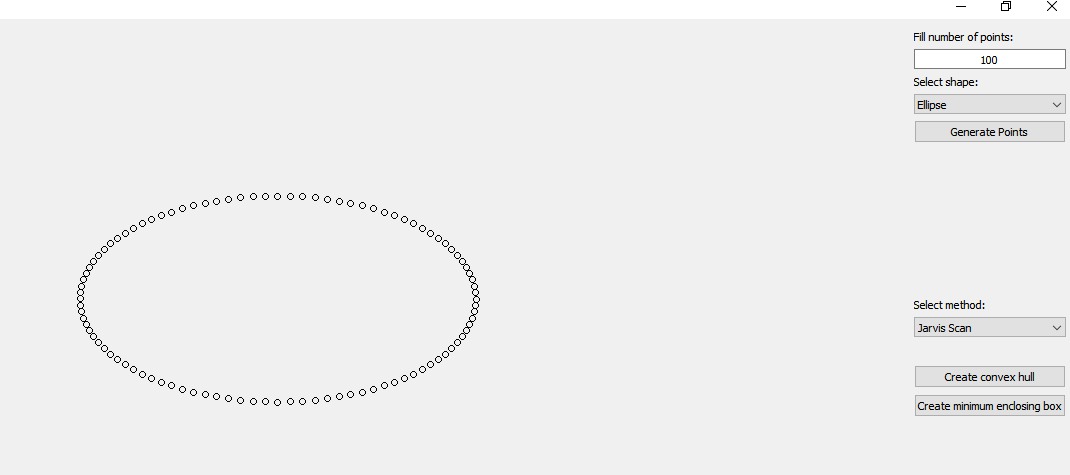
\includegraphics[width=14cm]{pictures/ellipse.png} 
\caption[Generování elipsy]{Generování elipsy}
\label{fig:ellipse}
\end{center}
\end{figure}
\vspace{-0.4cm}

%% -------<<< 3. KAPITOLKA = Problematické situace a jejich rozbor >>>-------\\%%
\newpage
\vspace*{-1cm}
\fancyhead[RE, RO]{\fancyplain{}{\small \sl{PROBLEMATICKÉ SITUACE A JEJICH ROZBOR}}}
\section{Problematické situace a jejich rozbor}
\subsection{Singulární případy u Jarvis Scan algoritmu}
U tohoto algoritmu dochází k určování maximálního úhlu ve vrcholu konvexní obálky. Podle tohoto kritéria je pak přidán další bod konvexní obálky. Je proto důležité, aby bod s tímto úhlem vždy jednoznačně nalezen. U pravidelných tvarů (např. mřížka) je ale mnoho bodů, ke kterým z daného bodu určíme stejný úhel, jelikož leží na stejné přímce. \\
\indent V rámci bonusové úlohy byla odstraněna tato singularita způsobena kolineárními body. Pokud je vypočtený úhel totožný nebo téměř totožný s aktuálně největším nalezeným úhlem, je vypočtena jednak vzdálenost od bodu konvexní obálky k bodu s maximálním úhlem, a jednak vzdálenost od bodu konvexní obálky k bodu s počítaným úhlem. Pokud je vzdálenost k počítanému bodu větší (je tedy dále na přímce), je tento bod označen jako bod s maximálním úhlem. Kolineární bod je tedy přeskočen a není zahrnut do polygonu konvexní obálky. Proto například polygon konvexní obálky zkontruovaný nad mřížkou, která se skládá se 100 bodů, bude mít pouze 4 body (ty, které ohraničují danou mřížku). Tato problematika je ošetřena ve zdrojovém souboru \textit{algorithms.cpp} na řádcích 118-126.
\subsection{Konstrukce striktně konvexních obálek}
U výsledných obálek můžou nastat následující singulární situace: 
\begin{enumerate}
\item bod konvexní obálky leží na úsečce mezi dvěma body konvexní obálky -- takový bod je nutné odstranit, 
\item na sobě leží dva identické body konvexní obálky -- jeden z nich je rovněž nutné odstranit.
\end{enumerate}
Oba tyto případy jsou řešeny na závěr každé z výše zmíněných funkcí na konstrukci konvexní obálky ve funkci \textit{correctCH}. K vymazání identických nebo téměř identických bodů byla definována třída \textit{isPointIdentical}, která definuje operátor totožnosti \textit{()}. Tento operátor pak vstupuje do funkce \textit{std::unique}, která vybere identické body, jež jsou v dalším kroku pomocí funkce \textit{erase} smazány z polygonu konvexní obálky.

\vspace{0.2cm}
\begin{figure}[hbt!] 
\begin{center}
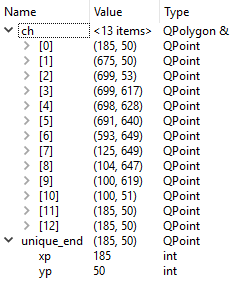
\includegraphics[width=6cm]{pictures/totozne.png} 
\caption[Případ dvou totožných bodů č. 11, 12 u konvexní obálky o 13 vrcholech]{Případ dvou totožných bodů č. 11, 12 u konvexní obálky o 13 vrcholech}
\label{fig:tot}
\end{center}
\end{figure}
\vspace{-0.4cm}

\begin{figure}[hbt!] 
\begin{center}
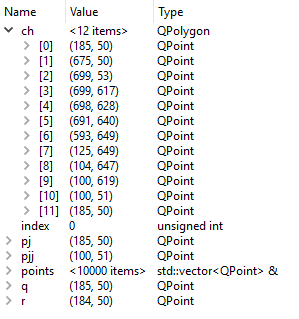
\includegraphics[width=6cm]{pictures/po_odstraneni.png} 
\caption[Situace po odstranění jednoho z identických bodů pomocí funkce \textit{std::unique}]{Situace po odstranění jednoho z identických bodů pomocí funkce \textit{std::unique}}
\label{fig:po_odstraneni}
\end{center}
\end{figure}
\vspace{-0.4cm}

Kolinearita bodů na stejné linii je řešena pomocí funkce \textit{getPointLinePosition}. Pokud je výstupem této funkce \textit{-1}, je daný bod na linii vymazán z polygonu konvexní obálky.

\subsection{Duplicity u Sweep Line algoritmu}
Problémy v této metodě mohou nastat v případě, že na vstupu budou duplicitní body. Tyto duplicity je tedy nutné ošetřit hned na začátku algoritmu:
\begin{enumerate}
\item Nalezení duplicitního bodu:  $ if( (points[j].x == points[i].x) \&\& (points[j].y == points[i].y) )$ 
\item Odstranění bodu z množiny: $ Delete$ $ points[i]$
\end{enumerate}
Tato problematika je ošetřena ve zdrojovém souboru \textit{algorithms.cpp} na řádcích 227-236.

\subsection{Singulární případy u Graham Scan algoritmu}
Podobně jako u Jarvis Scan algoritmu může nastat případ, že úhly k některým bodům jsou téměř totožné. Po setřídění bodů podle velikosti úhlů je tedy nutné spočítat rozdíl mezi počítaným úhlem a předchozím úhlem. Pokud je menší než zadaná tolerance, jsou počítány obě vzdálenosti od pivota směrem k bodu, který určuje pravé rameno počítaného úhlu, a od pivota směrem k bodu, který určuje pravé rameno předcházejícího úhlu. Pokud je vzdálenost k počítanému bodu větší (je tedy dále na přímce), je vzdálenost k předchozímu bodu nastavena na vzdálenost k počítanému bodu. Předcházející bod (ten s kratší vzdáleností) do polygonu konvexní obálky přidán není a do dalšího výpočtu není uvažován.
Tato problematika je ošetřena ve zdrojovém souboru \textit{algorithms.cpp} na řádcích 473-490.


%% -------<<< 4. KAPITOLA = Vstupní  data >>>-------\\%%
\newpage
\fancyhead[RE, RO]{\fancyplain{}{\small \sl{VSTUPNÍ A VÝSTUPNÍ DATA}}}

\vspace*{-1cm}
\section{Vstupní data}
Vstupní data tvoří analyzovaná skupina bodů datového typu std::vector<QPointF>, která je vygenerována po stisku tlačítka \textit{Generate Points}. Tento generátor vytváří pomocí funkce \textit{rand} množiny s předem definovaným počtem vrcholů a s předem definovaným typem (náhodná množina, rastr, kružnice, star-shaped polygon, elipsa).

%% -------<<< 2. KAPITOLA = Výstupní data >>>-------\\%%
\section{Výstupní data}
Hlavním výstupem této úlohy je grafická aplikace, která umožňuje nad vygenerovaným polygonem zkonstruovat konvexní obálku. Ke konstrukci je možné přistupovat pomocí čtyř různých metod -- Jarvis Scan, Quick Hull, Sweep Line či Graham Scan. Po stisku tlačítka \textit{Create convex hull} je výsledná obálka typu QPolygon zobrazena fialovou barvou a nad zmíněným tlačítkem je zobrazena doba běhu algoritmu. \\
\indent Ve chvíli, kdy je vytvořena obálka, může být po stisku tlačítka \textit{Create minimum enslosing box} vytvořen nejmenší možný ohraničující obdélník typu QPolygon. Ten je vykreslen tyrkysovou barvou. Hlavní směrová úsečka budovy typu QLineF je zobrazena tmavě modře.

%% -------<<< 3. KAPITOLA = Ukázka aplikace >>>-------\\%%
\newpage
\fancyhead[RE, RO]{\fancyplain{}{\small \sl{UKÁZKA APLIKACE}}}

\vspace*{-1cm}
\section{Ukázka aplikace}
\noindent
\large
Do této kapitolky je zahrnuto několik ukázek vytvořené aplikace. Zároveň s konstrukcí konvexních obálek a Minumum Enclosing Bounding Box jsou ukázany možnosti generátoru konvexních a nekonvexních množin.

\vspace{0.2cm}
\begin{figure}[hbt!] 
\begin{center}
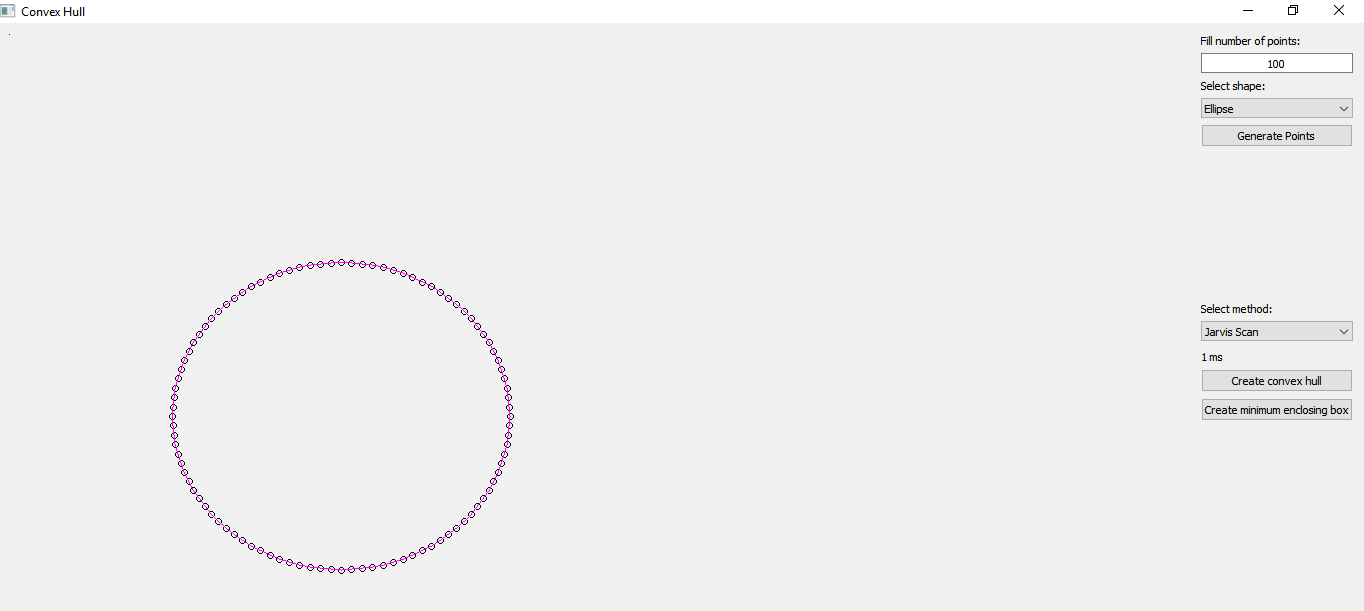
\includegraphics[width=15cm]{pictures/jarvis_ellipse.png} 
\caption[Konstrukce konvexní obálky metodou Jarvis Scan na elipse o 100 bodech]{Konstrukce konvexní obálky metodou Jarvis Scan na elipse o 100 bodech}
\label{fig:jar}
\end{center}
\end{figure}
\vspace{-0.4cm}

\vspace{0.2cm}
\begin{figure}[hbt!] 
\begin{center}
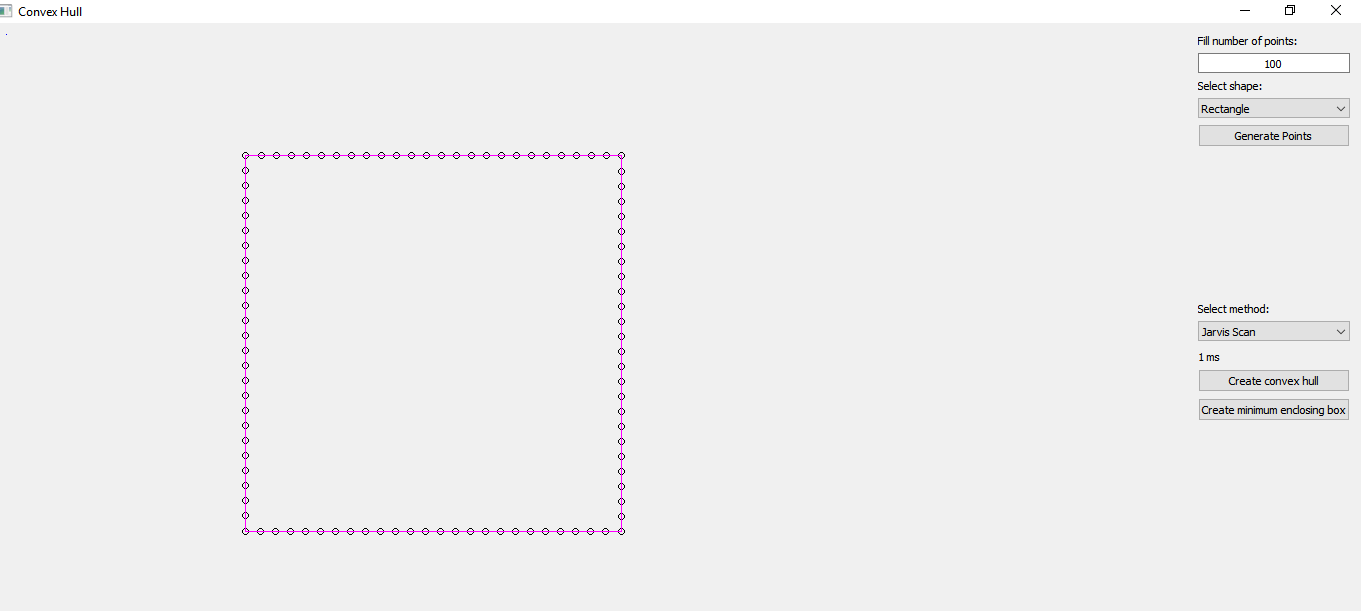
\includegraphics[width=15cm]{pictures/jarvis_rectangle.png} 
\caption[Konstrukce konvexní obálky metodou Jarvis Scan na obdélníku o 100 bodech]{Konstrukce konvexní obálky metodou Jarvis Scan na obdélníku o 100 bodech}
\label{fig:jarre}
\end{center}
\end{figure}
\vspace{-0.4cm}

\vspace{0.2cm}
\begin{figure}[hbt!] 
\begin{center}
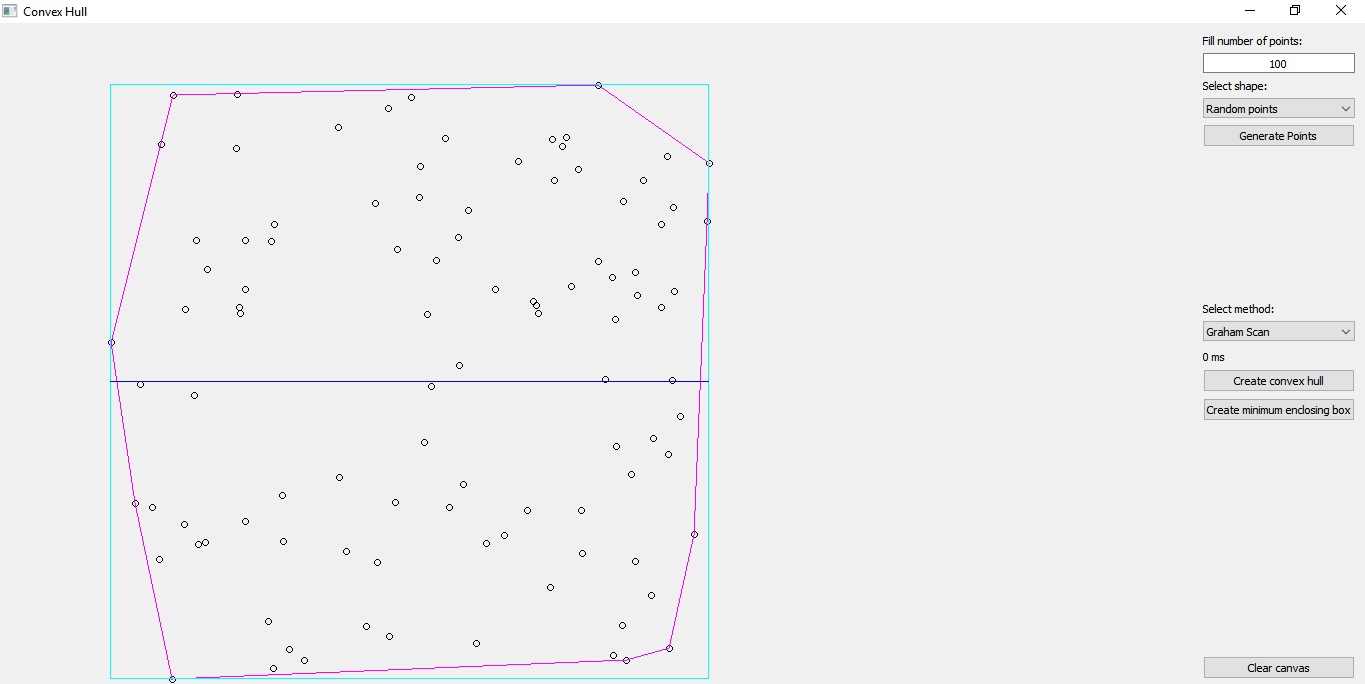
\includegraphics[width=15cm]{pictures/graham_random_enclosing_box.png} 
\caption[Konstrukce konvexní obálky metodou Graham Scan a Minimum Enclosing Box na náhodné množiny o 100 bodech]{Konstrukce konvexní obálky metodou Graham Scan a Minimum Enclosing Box na náhodné množině o 100 bodech}
\label{fig:enc}
\end{center}
\end{figure}
\vspace{-0.4cm}

\vspace{0.2cm}
\begin{figure}[hbt!] 
\begin{center}
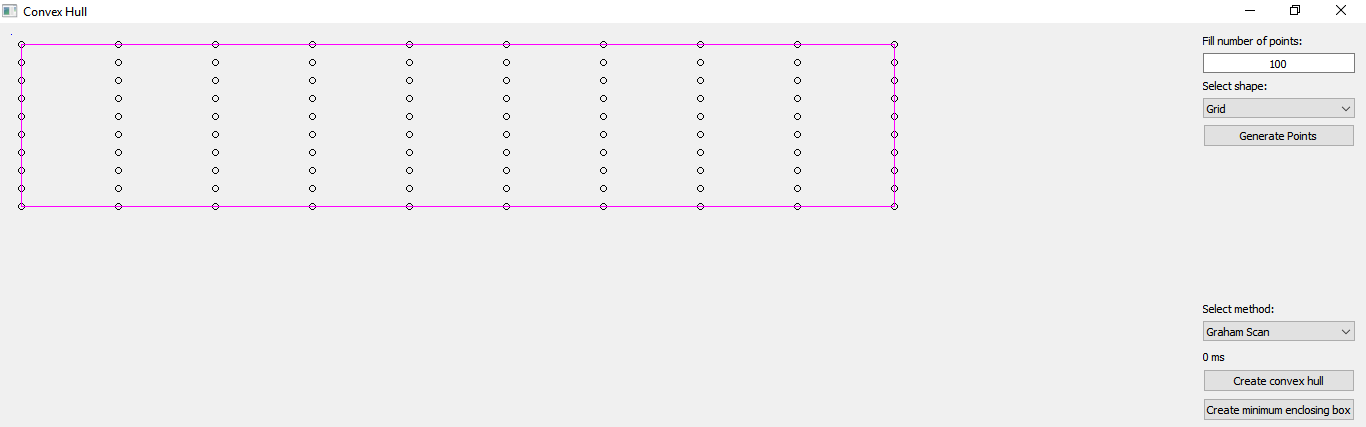
\includegraphics[width=14cm]{pictures/graham_grid.png} 
\caption[Konstrukce konvexní obálky metodou Graham Scan na pravidelné mřížce]{Konstrukce konvexní obálky metodou Graham Scan na pravidelné mřížce}
\label{fig:gr}
\end{center}
\end{figure}
\vspace{-0.4cm}

\begin{figure}[hbt!] 
\begin{center}
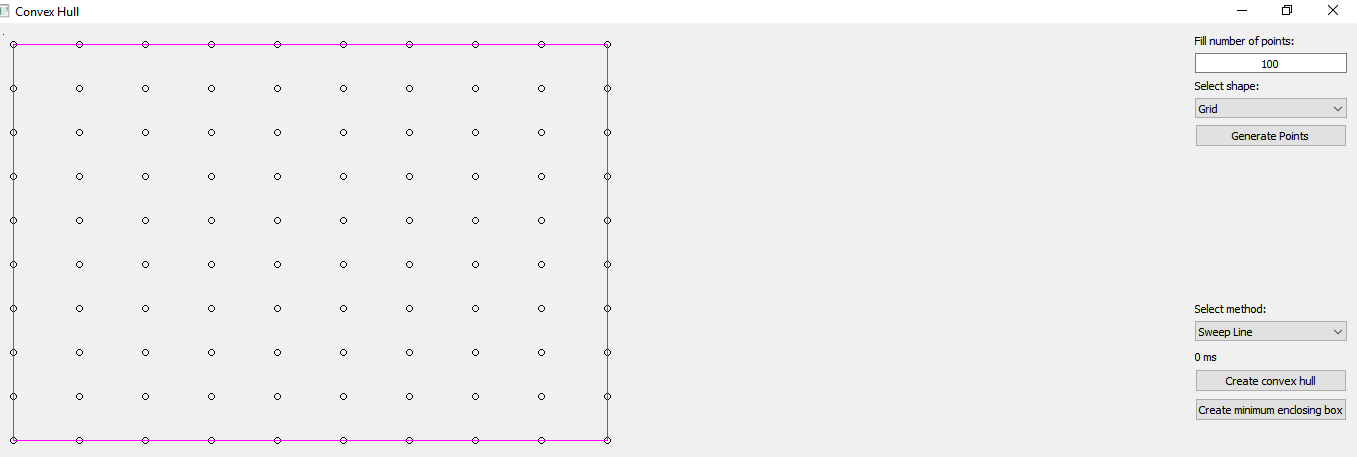
\includegraphics[width=14cm]{pictures/sweep_grid.png} 
\caption[Konstrukce konvexní obálky metodou Sweep Line na pravidelné mřížce]{Konstrukce konvexní obálky metodou Sweep Line na pravidelné mřížce}
\label{fig:sw}
\end{center}
\end{figure}
\vspace{-0.4cm}

\begin{figure}[hbt!] 
\begin{center}
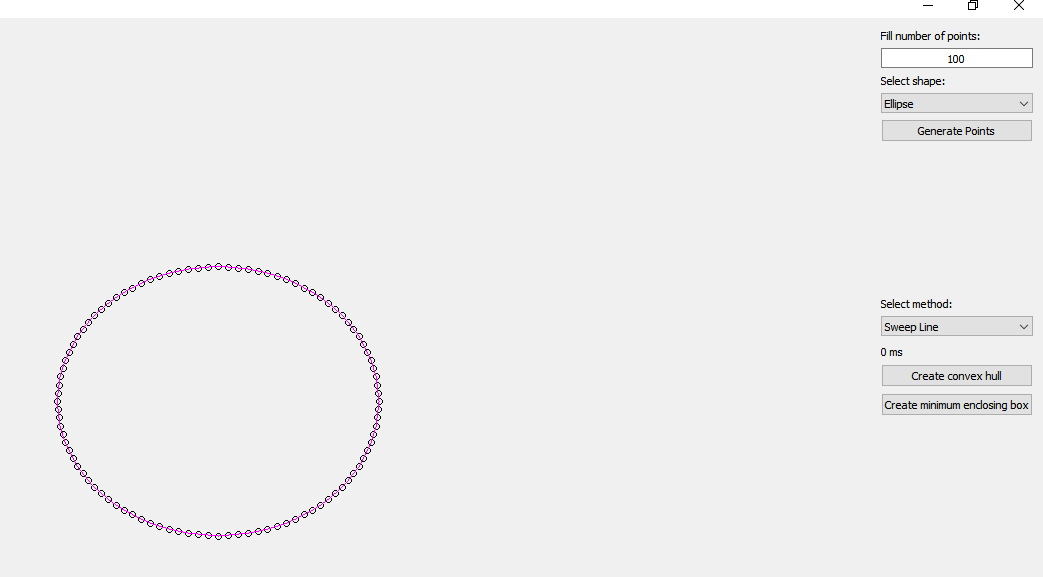
\includegraphics[width=14cm]{pictures/sweep_ellipse.png} 
\caption[Konstrukce konvexní obálky metodou Quick Hull na elipse]{Konstrukce konvexní obálky metodou Quick Hull na elipse}
\label{fig:qh}
\end{center}
\end{figure}
\vspace{-0.4cm}

\begin{figure}[hbt!] 
\begin{center}
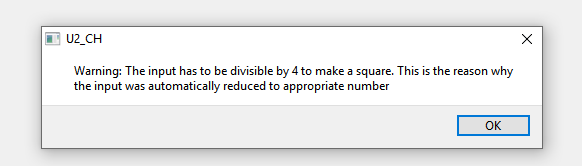
\includegraphics[width=12cm]{pictures/warning_rectangle.png} 
\caption[Varování u generování čtvercové množiny]{Varování u generování čtvercové množiny}
\label{fig:var}
\end{center}
\end{figure}
\vspace{-0.4cm}

\begin{figure}[hbt!] 
\begin{center}
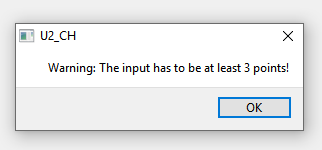
\includegraphics[width=8cm]{pictures/warning_ellipse.png} 
\caption[Varování u generování kruhu]{Varování u generování kruhu}
\label{fig:var2}
\end{center}
\end{figure}
\vspace{-0.4cm}


%% -------<<< 4. KAPITOLA = Technická dokumentace >>>-------\\%%

\newpage
\fancyhead[RE, RO]{\fancyplain{}{\small \sl{TECHNICKÁ DOKUMENTACE}}}

\vspace*{-1cm}
\section{Technická dokumentace}

\subsection{Struktury}
Ve zdrojovém souboru \textit{algorithms.cpp} je definována struktura, která přehledněji manipuluje s bodem, úhlem a vzdáleností.

\subsubsection{Angle}
Jedná se o strukturu, která definuje datový typ Angle, který je využíván v metodě Graham Scan. Skládá se z bodu q typu QPoint, z úhlu od rovnoběžky s osou x k tomuto bodu (double) a ze vzdálenosti mezi počátečním bodem a bodem q.

\subsection{Třídy}
V aplikaci se nachází celkem šest tříd - Algorithms, Draw, Generator, SortbyX, SortbyY a Widget. 

\subsubsection{Algorithms - pomocné metody}
Třída Algorithms je nejobsáhlejší. Obsahuje konstruktor a dalšich několik pomocných i hlavních metod, které jsou určeny pro výpočet algoritmů používaných v digitálním GIS. \\

\noindent\textbf{int getPointLinePosition(QPoint \&q, QPoint \&p1, QPoinF \&p2)}\\
Tato funkce má za úkol určit polohu bodu \textit{q} vůči přímce zadané dvěma body \textit{p1} a \textit{p2}. Z vektorů je vypočten determinant. Pokud je determinant větší než tolerance (1.0e-6), bod se nechází v levé polorovině a funkce vrací hodnotu \textit{1}. Pokud je menší než -tolerance, bod se nachází v pravé polorovině a funkce vrací hodnotu \textit{0}.  Pokud nenastane ani jeden z výše uvedených případů, tedy bod leží na linii, výstupem je hodnota \textit{-1}.\\

\noindent\textbf{double length2Points(QPoint p, QPoint q)}\\
Vrací vzdálenost dvou bodů vypočtenou z Pythagorovy věty.\\

\noindent\textbf{double getAngle2Vectors(QPoint \&p1, QPoint \&p2, QPoint \&p3, \\ QPoint \&p4)}\\
V této funkci je pomocí norem a skalárního součinu počítán úhel mezi dvěma hranami zadanými čtyřmi body typu QPoint. Úhel je vypočten jako arcus cosinus poměru skalárního součinu a součinu obou velikostí. Defaultně se v prostředí počítá v radiánech, což bylo ponecháno.\\

\noindent\textbf{double getPointLineDistance(QPoint \&q, QPoint \&p1, QPoint \&p2)}\\
Vrací vzdálenost bodu a přímky zadané dvěma body vypočtenou ze známých geometrických vzorců.\\

\noindent\textbf{void rotateByAngle(QPolygon \&points, double angle)}\\
Vrací vstupní polygon pootočený o daný úhel. Tato metoda je využívána při konstrukci Minimum Area Enclosing Box.\\

\noindent\textbf{void rotateByAngle(QLine \&points, double angle)}\\
Vrací vstupní linii pootočenou o daný úhel. Tato metoda je využívána při konstrukci Minimum Area Enclosing Box.\\

\noindent\textbf{QPolygon correctCH(QPolygon)}\\
Kontroluje, zda ve výsledné konvexní obálce nejsou téměř totožné body nebo kolineární body. Pokud ano, ošetří a vrátí opravenou konvexní obálku.

\subsubsection{Algorithms - hlavní metody}

\noindent\textbf{QPolygon jarvisScan(std::vector$<$QPoint$>$ \&points)}\\
Metoda pro výpočet konvexní obálky nad vstupní množinou bodů typu \textit{std::vector$<QPoint>$} algoritmem Jarvis Scan. Metoda vrací konvexní obálku s typem QPolygon.
\\

\noindent\textbf{QPolygon qHull(std::vector$<$QPoint$>$ \&points)}\\
Metoda pro výpočet konvexní obálky nad vstupní množinou bodů typu \textit{std::vector$<QPoint>$} algoritmem Quick Hull. Metoda vrácí konvexní obálku s typem QPolygon.
\\

\noindent\textbf{QPolygon qh(unsigned int s, unsigned int e, std::vector$<$QPoint$>$ \&points, QPolygon \&ch)}\\
Pomocná metoda pro rekurzi v metodě qHull. Na vstupu jsou indexy bodů s a e, které určují přímku, podle níž se určí, zda bod p patří do konvexní obálky H. Metoda nic nevrací, jen ukládá body, které patří do konvexní obálky.
\\

\noindent\textbf{QPolygon grahamScan((std::vector$<$QPoint$>$ \&points))}\\
Metoda pro výpočet konvexní obálky nad vstupní množinou bodů typu \textit{std::vector$<QPoint>$} algoritmem Graham Scan. Metoda vrácí konvexní obálku s typem QPolygon.
\\

\noindent\textbf{QPolygon sweepLine((std::vector$<$QPoint$>$ \&points))}\\
Metoda pro výpočet konvexní obálky nad vektorem bodů metodou Sweep Line. Metoda vrácí konvexní obálku s typem QPolygon.
\\

\noindent\textbf{QPolygon minimumAreaEnclosingRectangle(QPolygon \&ch, QPolygon \&rectangle, QLine \&direction)}\\
Metoda pro výpočet hlavních směrů budovy. Na vstupu je konvexní obálka ch a prázdné proměnné rectangle a direction. Do rectangle se uloží minimální ohraničující obdélník a do direction hlavní směr budovy.

\subsubsection{Generator}
Třída Generator obsahuje různé metody, které automatizovaně vrací různé konvexní či nekonvexní množiny bodů různých tvarů. \\

\noindent\textbf{std::vector\textless QPoint \textgreater generateCircle(int n)}\\
Metoda generuje výstupní množinu bodů ve tvaru kruhu. Na vstupu je počet generovaných bodů. Návratová hodnota je vektor bodů.\\

\noindent\textbf{std::vector\textless QPoint \textgreater generateEllipse(int n)}\\
Metoda generuje výstupní množinu bodů ve tvaru elipsy. Na vstupu je počet generovaných bodů. Návratová hodnota je vektor bodů.\\

\noindent\textbf{std::vector\textless QPoint \textgreater generateSquare(int n)}\\
Metoda generuje výstupní množinu bodů ve tvaru čtverce. Na vstupu je počet generovaných bodů, pokud není dělitelný čtyřmi je počet upraven. Návratová hodnota metody je vektor bodů.\\

\noindent\textbf{std::vector\textless QPoint \textgreater generateStarShape(int n)}\\
Metoda generuje výstupní množinu bodů ve tvaru hvězdy. Na vstupu je počet generovaných bodů. Návratová hodnota je vektor bodů.\\

\noindent\textbf{std::vector\textless QPoint \textgreater generateRandomPoints(int n)}\\
Metoda generuje množinu náhodně rozmístěných bodů. Na vstupu je počet generovaných bodů. Návratová hodnota je vektor bodů.\\

\noindent\textbf{std::vector\textless QPoint \textgreater generateGrid(int n)}\\
Metoda generuje pravidelnou mřížku. Na vstupu je počet generovaných bodů.  Pokud není odmocnina celé číslo, je počet upraven, tak aby odmocninou celé číslo bylo. Návratová hodnota metody je vektor bodů.

\subsubsection{SortbyX}
Třída, která definuje operátor přetížení \textit{()}, který třídí body podle X souřadnice. Pokud je X souřadnice stejná, rozhoduje se podle souřadnice Y.

\subsubsection{SortbyY}
Třída, která definuje operátor přetížení \textit{()}, který třídí body podle Y souřadnice. Pokud je Y souřadnice stejná, rozhoduje se podle souřadnice X.

\subsubsection{SortbyAngle}
Třída, která definuje operátor přetížení \textit{()}, který třídí úhly typu Angle (samostatně definovaná struktura) podle velikosti. Pokud je úhel stejný, rozhoduje vzdálenost mezi datovými prvky typu Angle.

\newpage
\vspace*{-1cm}
\subsubsection{Draw}
Třída Draw dědí od třídy QWidget. \\

\noindent\textbf{void mousePressEvent}\\
V této funkci je vykreslen bod \textit{q} a je přidán do vektoru bodů \textit{points}\\

\noindent\textbf{void paintEvent}\\
Tato metoda slouží k vykreslení bodů \textit{points}. Zároveň je díky této metodě vykreslena konvexní obálka a minimum enclosing box spolu s hlavním směrem budovy.\\

\noindent\textbf{void clearCanvas}\\
Metoda sloužící k vymazání všech polygonů i bodů a k překreslení. Volá se před automatickým generováním vstupní množiny. \\

\noindent\textbf{void clearCanvas}\\
Metoda sloužící k vymazání všech polygonů i bodů a k překreslení. Volá se před automatickým generováním vstupní množiny. \\

\noindent\textbf{QPoint getPoints}\\
Metoda, která vrací privátní body \textit{q} třídy Draw.\\

\noindent\textbf{QPoint getConvexHull}\\
Metoda, která vrací privátní konvexní obálku \textit{P} třídy Draw, aby bylo možné ji vracet ve třídě Widget. \\

\noindent\textbf{QPoint  setCH}\\
Metoda, která naopak vektor konvexní obálky, který je vytvořen ve třídě Widget, uloží do privátních datových typů ve třídě Draw.
Obdobně pracují i další veřejné metody \textbf{QPoint  setPoints}, \textbf{QPoint  setBox} a \textbf{QPoint  setDirection}.

\newpage
\vspace*{-1cm}
\subsubsection{Widget}
\noindent\textbf{void on\_create\_CH\_clicked}\\
Při stisknutí tohoto tlačítka se v závislosti na vybrané variantě algoritmu v Comboboxu, provede daný výpočet. A výsledek se předá třídě Draw pro vykreslení. Je zde také měřen čas jednotlivých algoritmů pomocí funkce \textit{std::clock}.\\

\noindent\textbf{void on\_quit\_clicked}\\
Při stisknutí tlačítka Quit je uživateli vyzván, zda si přeje ukončit aplikaci. Pokud stikne OK, aplikace se ukončí.\\

\noindent\textbf{void on\_clear\_clear\_clicked}\\
Při stisknutí tlačítka Clear se zavolá metoda třídy Draw clearCanvas.\\

\noindent\textbf{void on\_generate\_clicked}\\
Při stisknutí tohoto tlačítka přivolána metoda generatePolygon, která podle zadaného počtu vrcholů vykreslí nekonvexní polygon.\\

\noindent\textbf{void on\_minimum\_enclosing\_box\_clicked}\\
Při stisknutí tlačítka se nad konvexní obálkou zavolá metoda třídy Algorithms minimumAreaEnclosingRectangle.

\section{Testování}
Testování bylo prováděno v režimu Release a bylo testováno chování všech čtyřech algoritmů. Testování je k dispozici v přiloženém souboru \textbf{testování.xlxs}. V tomto souboru jsou u všech algoritmů voleny typy vstupních množin kruh, mřížka a náhodné rozmístění. V každé ze záložek je vždy rozebrán jeden konrétní algoritmus a doby běhu jsou jednak vyplněny v tabulce, a jednak znázorněny do příslušného grafu. Testování pro daný počet bodů bylo provedeno vždy desetkrát. Výsledná doba běhu algoritmu je vypočtena jako průměr. Jelikož máme více měření, bylo možné určit i varianci. Poslední záložka obsahuje porovnání časové náročnosti všech algoritmů pro jednotlivé typy vstupních množin.

%% -------<<< 5. KAPITOLA = Závěr >>>-------\\%%
\newpage
\fancyhead[RE, RO]{\fancyplain{}{\small \sl{ZÁVĚR}}}

\vspace*{-1cm}
\section{Závěr}
\noindent
\large
V rámci úlohy byla vytvořena aplikace, která je schopna na vygenerovaných bodech zkonstruovat konvexní obálku. Zároveň je v rámci aplikace možné náhodně vygenerovat vstupní množiny bodů a to do šesti různých tvarů, což uživatel jistě ocení.\\
\indent Součástí úlohy bylo i testování doby výpočtu jednotlivých konvexních obálek. U všech algoritmů je zahrnuta funkce, která opravuje singulární případy, tuto funkci tedy musíme do výsledné body běhu připočíst. \\
\indent Nyní je na čase shrnout výsledky testování. Algoritmus Jarvis Scan měl znatelně nejhorší čas, a to zejména pro vstupní množinu ve tvaru kruhu, kdy se průměrná doba běhu pro množinu o milionu bodech pohybovala kolem 25000 ms. Naopak metoda Sweep Line se zdá býti nejlepším řešením, a to pro všechny typy vstupních množin. Sweep Line má velmi krátkou dobu běhu i pro kruhovou množinu, kdy Quick Hull poněkud zaostává. Jinak jsou algoritmy Sweep Line a Quick Hull srovnatelné. Metoda Graham Scan je o trochu pomalejší, ale má vyrovnanou dobu běhu pro všechny vyzkoušené typy vstupních množin.

\subsection{Náměty na vylepšení}
\large
\begin{itemize}
\item Celý skript by mohl být převeden do floating point number datových typů, jelikož přetypovávání na integery v rámci odstranění warningů je poněkud krkolomné. Bohužel prvotním nápadem bylo používat datové typy QPointF, QLineF, QPolygonF, funkce Quick Hull však padala z důvodu špatné segmentace. Tuto chybu se vyřešit nepodařilo, pravděpodobně souvisí se složitostí rekurzivní metody. Body ze vstupní množiny byly tedy generovány s datovým typem QPoint.
\item V rámci úlohy bylo provedeno mnoho testování pro různý počet bodů, různý typ vstupní množiny a různý algoritmus. Za úvahu by určitě stálo, popřemýšlet o vhodné automatizaci.  Autorce se bohužel nedaří spustit výsledný exe soubor, aplikace hlásí chybu Kód nelze spustit, protože se nenašel Qt5Cored.dll... I když byla snaha tuto chybu opravit, nepodařilo se. Volání takového exe souboru odkudkoli by kvůli této chybě také zřejmě nefungovalo. Proto žádná automatizace nakonec implementována nebyla.\\
\indent Nicméně, pokud by bylo zaručeno, že exe soubor lze bezchybně spustit a zavolat s příslušnými parametry, určitě by časová úspora testování byla velmi výrazná. Vzhledem k tomu, že autorka má zkušenosti se psaním Powershell skriptů, nebyl by problém v rámci takového skriptu nadefinovat tři argumenty - typ vstupní množiny, počet generovaných bodů vstupní množiny a typ algoritmu ke konstrukci konvexní obálky. V Powershell skriptu by se poté v několika for cyklech volal .exe soubor s příslušnými argumenty.\\
\indent Autorka má již zkušenosti s voláním Python skriptu s argumenty v Powershellu. V Pythonu je možné celkem jednoduše nadefinovat pomocí knihovny argparse argumenty, které je pak možné Python skriptu předat právě například pomocí Powershellu nebo jen v obyčejném .bat souboru. \\
\indent V Qt by bylo možné vytvořit něco obdobného a to pomocí třídy QCommandLineParser, kterou je třeba přidat do zdrojového souboru main.cpp klauzulí \textit{$\#include <QCommandLineParser>$}. Uvnitř funkce main je poté nutné nadefinovat vstupní parametry a předat je třídě widget. Výsledné doby běhu jednotlivých algoritmů by mohly být dále vyexportovány spolu s označením použitých argumentů do textového souboru.
\end{itemize}
 

%% -------<<< LITERATURA >>>-------\\%%
\newpage
\vspace*{-6ex}
\renewcommand{\refname}{Literatura} 
\fancyhead[RE, RO]{\fancyplain{}{\small \sl{LITERATURA}}}
    \bibliographystyle{czechiso}
    \bibliography{literatura}
 
\end{document}


